%===================== CROSS-MEDIA LEARNING FOR IMAGE CLASSIFIERS =========================

\graphicspath{{img/vsa/}}

\newcommand{\BTSA}{B-T4SA}
\newcommand{\ourFtAlex}{Hybrid-T4SA}
\newcommand{\ourFtVGG}{VGG-T4SA}

\chapter{Weakly-supervised Cross-media Learning of Convolutional Neural Networks}
\label{ch:cross-media}

The most straightforward way to build a visual image classifier using \glspl{cnn} is to perform supervised learning.
While in previous work the cost of human interaction was spent on the manual engineering of features detectors and descriptors, this cost recently shifted to the labeling of datasets in order to train deep models.
Even if the labeling task is simpler and more accessible, correctly labeling huge datasets is still a labor-intensive and expensive job, which is usually carried out by crowd-sourcing.
Current large-scale datasets, such as ImageNet, are in fact limited in their scalability due to the labeling cost on which their collectors incur.
Thus, the attention of recent research shifted to the exploitation of the huge amount of data coming from the web and social media which became easily available in the last years~\cite{sun2017revisiting,mahajan2018exploring}.
The main objective is to reduce the amount of human interaction needed to train an image classifier and obtain good features by exploiting correlation that can emerge in large-scale datasets.
Despite having the advantage of being free and constantly growing, this source of data poses challenges in its usage, since it commonly presents noisy or incomplete information.
This usually limits the amount of supervision that can be extracted from this kind of data, but the possibility to scale the training procedures to a huge amount of data often compensates this limitation.

In this chapter, we propose a novel weakly-supervised cross-media approach to train visual image classifiers in an autonomous way exploiting social media data.
We rely on textual data --- which usually accompanies images in social media posts --- to provide a noisy supervision in the training phase of a visual-only classifier.
To exhibit the advantages of our approach, we employed it to tackle \emph{\gls{vsa}} --- a problem in which the cost of data labeling is rather high --- using a \acrfull{dcnn} trained without relying on any hand-assigned ground-truth.
We present an empirical study to analyze visual sentiments in the wild, starting from a large-scale dataset of \emph{unlabeled} user-generated content.
To the best of our knowledge, this is the first work that proposes a cross-media approach to learn a classifier for predicting the sentiment polarity of a given image.
We demonstrate via experimental evaluation on existing manually-labeled benchmarks that models trained with our approach are able to extensively exploit the noisy information contained in uncontrolled social media data to build a visual sentiment polarity classifier with no human supervision that outperforms state-of-the-art classifiers trained on sentiment-related labeled images.
Overall, we collect and analyze more than 3 million tweets from which we build \emph{\acrfull{t4sa}} --- a dataset of about 1 million high-confidence tweets, for which we provide the textual sentiment classification, and the corresponding 1.4M images.
We make all the collected tweets, the \gls{t4sa} dataset, and trained models publicly available to foster new research on the field of visual sentiment analysis.

The chapter is structured as follows.
In \ref{sec:vsa:introduction}, the problem of visual sentiment analysis is presented, together with a discussion about the challenges it poses and an overview of the current state of the art.
\ref{subsec:vsa:dataset} presents the methodology used to collect and preprocess the social media data used in our experiments.
In \ref{subsec:vsa:method}, our weakly-supervised cross-media learning approach is described in detail, and \ref{sec:vsa:experiments} reports its experimental evaluation and comparison with state-of-the-art approaches to visual sentiment analysis.
\ref{sec:vsa:conclusion} summarizes the main findings and concludes the chapter.

The research presented in this chapter was published in~\cite{vadicamo2017cross}, and the provided resources --- e.g., datasets and trained models --- are available at \url{http://t4sa.it}.


%%% ABSTRACT
% Much progress has been made in the field of sentiment analysis in the past years. Researchers relied on textual data for this task, while only recently they have started investigating approaches to predict sentiments from multimedia content.
%With the increasing amount of data shared on social media, there is also a rapidly growing interest in approaches that work ``in the wild'', i.e., that are able to deal with uncontrolled conditions.
%In this work, we faced the challenge of training a visual sentiment classifier starting from a large set of user-generated and unlabeled contents.
%In particular, we collected more than 3 million tweets containing both text and images, and we leveraged on the sentiment polarity of the textual contents to train a visual sentiment classifier.
%To the best of our knowledge, this is the first time that a cross-media learning approach is proposed and tested in this context.
%We assessed the validity of our model by conducting comparative studies and evaluations on a benchmark for visual sentiment analysis.
%Our empirical study shows that --- although the text associated to each image is often noisy and weakly correlated with the image content --- it can be profitably exploited to train a deep Convolutional Neural Network that effectively predicts the sentiment polarity of previously unseen images.

\section{Visual Sentiment Analysis}
\label{sec:vsa:introduction}

Recent years experienced a rapid and increasing adoption of social media as information exchange and communication platforms.
On a daily basis, users generate and share a large quantity of multimedia content --- such as texts, images, and videos --- which conveys information about their opinions about a vast range of topics.
The availability of such a source of data attracted the scientific community as well as the industries to large-scale sentimental analyses of the public opinion.
Opinion mining and sentiment analysis~\cite{pang2008opinion} foster applications in multiple domains, such as market prediction~\cite{mishne2006predicting,asur2010predicting}, government intelligence~\cite{abbasi2007affect}, political elections~\cite{laver2003extracting,o2010tweets}, and crisis management~\cite{avvenuti2016impromptu,cresci2015linguistically}, to name a few.

Thanks to the multi-modality of modern social platforms, current trends show that visual media are increasingly chosen due to their immediate and effective communication, and less and less text is written by users.
Therefore, researchers shifted their attention from a pure textual-based sentiment analysis presented in seminal work to a multi-modal analysis which includes also visual information conveyed by images and videos~\cite{borth2013large,cao2016cross,jou2015visual,siersdorfer2010analyzing,you2015robust,you2016cross}.
In particular, we identify as \emph{visual sentiment analysis} the task of extracting subjective information --- such as emotions and opinions --- solely from visual data.
Understanding the content of a piece of visual information is an objective task, and much progress has been made in the computer vision research community to accurately describe visual contents, i.e., reducing the semantic gap between image representations and content~\cite{li2016socializing}.
However, describing the emotions arisen in human observers is challenging due to the high subjectivity involved.
This discrepancy between the affective content of an image and its description --- known as the \emph{affective gap}~\cite{siersdorfer2010analyzing} --- poses considerable challenges to visual sentiment analysis.
This difficulty is also reflected in the generation of labeled sets for training sentiment classifiers;
several emotional judgments by multiple annotators are usually required to obtain a high-quality sentiment ground-truth for a single image, thus increasing the cost of dataset creation.

While in general sentiment analyses can tailor a large range of emotions, the commonly adopted form of sentiment analysis is the determination of the sentiment polarity of a piece of information, i.e., an indicator of the emotional positiveness or negativeness conveyed.
This formulation is often sufficient for most sentiment analysis applications while simplifying the problem to be solved.
As the vast majority of attempts in the literature, we adopt the same formulation in our work;
thus, our goal is to predict the sentiment polarity of a given image.
In the next paragraphs, we will provide the reader with an overview of existing work on sentiment analysis with emphasis on the ones based on visual data.

\paragraph{Text-based Sentiment Analysis}
%For what concerns the detection of sentiment polarity in texts extracted from Twitter, first works considered simple linguistic features, such as word unigrams, word bigrams and parts-of-speech, using machine learning algorithms like Naive Bayes, Maximum Entropy and \acrfullpl{svm}.
Seminal works on sentiment polarity estimation from textual data~\cite{go2009twitter,bermingham2010classifying} employed classic \gls{ml} algorithms which relied on simple linguistic features --- such as word n-grams and part-of-speech.
%In the last few years, deep neural networks contributed to considerable performance improvements with respect to other popular learning algorithms, such as \glspl{svm}.
Subsequently, deep learning approaches positively contributed with more accurate models for text analysis and natural language processing, which in turn gave a huge contribution in textual sentiment analysis.
%In particular, \acrfullpl{lstm}, which we also employ in this work, and \acrfullpl{cnn} were tested on several shared tasks, such as the Semeval Sentiment analysis in Twitter \cite{nakov2016semeval}, which is considered by the Natural Language Processing community the most important benchmark for this task.
%The results obtained by the submitted systems, such as the ones by \citet{deriu2016swisscheese} and \citet{rouvier2016sensei}, have shown that the combination of these learning techniques with the adoption of word embeddings, a compact real-value vector word representation which takes into account word similarity \cite{mikolov2013distributed,pennington2014glove}, is able to set the state-of-the-art with minimal feature engineering, which makes such architectures more robust and flexible than previous ones.
The Semeval Sentiment analysis in Twitter \cite{nakov2016semeval} challenge is a testimony of this influence: an increasing number of submitted solutions~\cite{deriu2016swisscheese,rouvier2016sensei} combined the power of deep models --- such as \acrfullpl{lstm} and \acrfullpl{cnn} --- and word embeddings~\cite{mikolov2013distributed,pennington2014glove} to set the state of the art with minimal or no feature engineering.

% ---

\paragraph{Visual Sentiment Analisys}
In comparison to textual-based sentiment analysis, inferring emotional information from visual content has been less explored by the research community.
Seminal approaches \cite{machajdik2010affective,siersdorfer2010analyzing,jia2012can} relied on supervised or semi-supervised frameworks that map low-level features of images into human emotions.
\citet{siersdorfer2010analyzing} firstly applied and evaluated automatic classification of the sentiment using a large-scale collection of photos crawled from Flickr using the SentiWordNet \cite{esuli2007sentiwordnet} dictionary as query terms.
They used a pixel-level color histogram and \gls{sift}-based \acrlong{bow} representations as visual features and trained a \gls{svm} to predict the sentiment of images.
% To overcome the \emph{affective gap} between low-level features and the emotional content of an image,  employed visual entities or attributes to extract mid-level visual representations.
% The main contribution of~\cite{borth2013large} and~\cite{jou2015visual} was building a large scale visual sentiment ontology, called VSO and Multilingual VSO, respectively, which consist of thousands of semantic objects (Adjective Noun Pairs -- ANP) strongly linked to emotions.
% Using their ontologies, they also proposed a bank of detectors, namely \emph{SentiBank} and \emph{MVSO}, that can automatically extract these mid-level representations.
Subsequent works \cite{borth2013large,yuan2013sentribute,jou2015visual} proposed to employ large-scale sentiment ontologies --- like VSO~\cite{borth2013large} or MVSO~\cite{jou2015visual} --- comprised by emotion-related concepts identified by adjective-noun pairs.
%For example, Sentibank detects the responses of 1200 ANP concepts in an image, which means that it represents each image by a 1200-dimensional vector of responses.
%For the sentiment prediction task, a classifier is learned on the top of these mid-level representations that are used as image features.
Ontologies are used to build a feature extractor --- called \emph{SentiBank} --- which creates a mid-level visual representation based on the visual detection of these concepts, on which in turn the sentiment prediction relies.
%\citet{chen2014deepsentibank} proposed an improved version of SentiBank, called \emph{DeepSentiBank} which exploit \acrfullpl{dcnn} to build a visual sentiment concept classification model.
\citet{chen2014deepsentibank} extended this approach proposing \emph{DeepSentiBank}, in which the concept detection is carried out by deep convolutional models.
%Following the success of deep learning, many other approaches based on deep neural networks have been proposed for visual sentiment prediction and image emotion classification \cite{campos2017pixels,chen2014deepsentibank,islam2016visual,rao2016learning,you2015robust,xu2014visual}.
Many other approaches employed \glspl{dcnn} for visual sentiment prediction and image emotion classification~\cite{campos2017pixels,chen2014deepsentibank,islam2016visual,rao2016learning,you2015robust,xu2014visual}.
% ---
Most of these have in common the use of \glspl{cnn} trained or fine-tuned on sentiment-related and labeled data.
In \cite{campos2017pixels,chen2014deepsentibank,islam2016visual,jou2015visual}, %,xu2014visual %sun2016discovering %VGGNet \cite{simonyan2014very}
state-of-the-art \gls{cnn} architectures --- such as AlexNet~\cite{krizhevsky2012imagenet}, PlaceCNN~\cite{zhou2014learning}, and GoogleNet \cite{szegedy2015going} --- were exploited.
\citet{you2015robust} proposed a custom \gls{cnn} architecture specifically designed for visual sentiment prediction.
Since their network was trained on weakly labeled images, they also proposed an approach, called PCNN, to reduce the impact of noisy training images. %instances by progressively select a subset of the training images.
\citet{sun2016discovering} boosted the performance of CNNs by selecting affective local regions of the images which are likely containing objects and carrying massive emotions. % NOELAB
% This means that the ANP's textual sentiments are not explicitly used for the sentiment prediction.
Just recently, \citet{li2018image} investigated the fusion of the sentiment prediction obtained using visual ontologies with the sentiment prediction obtained using the textual sentiment values of adjective-noun pairs on which ontologies are built.


\paragraph{Multi-modal Sentiment Analysis}
There are also several publications on analyzing sentiments using multi-modalities, such as text and image.
For example, \citet{cao2016cross} proposed a late fusion to combine the predictions obtained from text and image, while \citet{you2016cross} proposed a cross-modality consistent regression (CCR) scheme for joint textual and visual analysis.
Recently, multi-modal learning approaches have been proposed for joint textual and visual understanding.
\citet{baecchi2016multimodal} proposed a multi-modal feature learning schema based on CBOW and denoising autoencoders to perform sentiment analysis.
In \cite{mao2014deep}, the authors proposed a deep end-to-end architecture where each modality is encoded is an appropriate sub-network (an \gls{rnn} for text and a \gls{cnn} for images) and then fused in a multi-modal layer.
Similarly, \citet{ma2015multimodal} encodes both modalities with convolutional networks.

Differently from all the approaches previously presented, in our work we are interested in i) understanding human sentiments by exploiting a large-scale dataset of unlabeled images collected from social-media, ii) training sentiment classifiers without any prior knowledge of the collected data.
Although textual information accompanying social media images is often incomplete and noisy, it can be effectively exploited to enable unsupervised sentiment analysis.
A first step in this direction was taken in \cite{wang2015unsupervised} where an Unsupervised SEntiment Analysis (USEA) for social-media images based on nonnegative matrix factorization was proposed.
Our work differs from that of \citet{wang2015unsupervised} in the final classifier and in the way in which we exploit the textual information.
In fact, we train a deep neural network that can be used to predict the sentiment of any new image \emph{without} using any textual information for those images, while USEA infers sentiments for images by \emph{jointly} considering visual and textual information.
%Moreover, Wang \etal  did not test their approach on hand-labeled images or benchmarks for visual sentiment analysis for further comparisons.

%-------------------------------------------------------------------------

\section{Learning Visual Sentiment Classifiers}

We focus our investigation on training a model to predict the sentiment polarity of a given image.
We formulate this task as learning a three-way image classifier that can assign either \emph{positive}, \emph{negative} or \emph{neutral} label to an image.
As other state-of-the-art approaches, we exploit deep learning models to build our visual sentiment classifiers.
However, differently from previous supervised approaches, we propose an end-to-end pipeline to train the visual classifier starting from a large-scale dataset of unlabeled tweets.
As source of multi-modal information, we choose Twitter, from which we crawled tweets from the random stream of global tweets with a minimum set of restriction.
We exploit the correspondence of text and images present in tweets to distill affective information from the textual modality to the visual one.
In particular, we use a pre-trained textual predictor --- based on a tandem \gls{LSTM}-\gls{SVM} architecture --- to infer the sentiment polarity from the textual part of a tweet
Then, we transfer this sentiment polarity to the images attached to the same tweet, obtaining a dataset of labeled images we can use as training set to fine-tune \glspl{dcnn} architectures for the task of visual sentiment polarity prediction.
Although the text of the tweets is often noisy or misleading with respect to the image content (e.g., irrelevant comments), we show that our cross-media approach can be profitably used for learning visual sentiment classifiers in the wild.
At test time, the trained \glspl{dcnn} can be used to infer the sentiment polarity of an image without the need of textual data.

In the next sections, we will describe the data collection process, the pre-trained textual sentiment classifier that provides us with weak supervision, and the training process of visual models.
%An overview of our approach is depicted in \ref{fig:vsa:overview}.
% TODO [FIGURE] VSA overview
%\begin{figure}
%    \centering
%    \includegraphics{}
%    \caption{.}
%    \label{fig:vsa:overview}
%\end{figure}

% We follow the current trend of facing sentiment ``in the wild", that is, in all sort of varying conditions of the everyday world that we share with others (as opposed to testing situation in laboratories).
% For this scope, social networks, such as Twitter and Facebook, are particularly suitable as sources of data for our analysis, thanks to the huge variation of contents shared by their users.

%-------------------------------------------------------------------------

\subsection{Data Collection}
\label{subsec:vsa:dataset}
Both the textual and the multimedia data used in this work have been collected from Twitter, by means of a streaming crawler.
The data collection process took place from July to December 2016, lasting around 6 months in total.
During this time span, we exploited Twitter's Sample API\footnote{https://dev.twitter.com/streaming/reference/get/statuses/sample} to access a random 1\% sample of the stream of all globally produced tweets.
All the tweets collected undergone a filtering step in order to retain only data that could be useful for our sentiment analysis task.
Specifically, we discarded: i) retweets; ii) tweets not containing any static image (i.e., we also discarded tweets containing only videos and/or animated GIFs); iii) tweets not written in the English language; iv) tweets whose text was less than 5 words long.
This ensures that we collect tweets with both images and text, and that there is enough textual data for the textual sentiment classification task.
Discarding retweets avoids collecting large numbers of duplicated images.
The above set of rules filtered as much as 98.7\% of all the tweets collected from the Twitter stream.
Anyway, the huge volume of tweets produced globally still allowed to collect a stream of more than 43 useful tweets per minute, on average.
At the end of the data collection process, the total number of tweets in our dataset is roughly 3.4M, corresponding to roughly 4M images.
Then, we classified the sentiment polarity of the \emph{texts} as described in the next section, and we selected the tweets having the most confident textual sentiment predictions to build our \emph{\acrfull{t4sa}} dataset.
\gls{t4sa} contains little less than a million tweets, corresponding to roughly 1.5M images.
We publicly release all the collected tweets and the \gls{t4sa} dataset.

%-------------------------------------------------------------------------

\subsection{Inferring Sentiment Polarity from Text}
\label{subsec:vsa:method}

The text extracted from the collected tweets has been classified according to the sentiment polarity using an adapted version for the English language of the ItaliaNLP Sentiment Polarity Classifier~\cite{cimino2016tandem}.
This system was successfully employed in the SENTIment POLarity Classification task~\cite{barbieri2016overview}, which was organized within Evalita 2016, the 5th evaluation campaign of Natural Language Processing and Speech tools for Italian.
This classifier is based on a tandem LSTM-SVM architecture.
\gls{svm} classifiers usually rely on ``sparse" and ``discrete" features in document classification tasks, making difficult the detection of relationships in sentences, which is often the key factor in detecting the overall sentiment polarity in documents~\cite{tang2015document}.
On the contrary, \glspl{lstm} were recently tested on Sentiment Analysis and proved to outperform previous systems~\cite{nakov2016semeval} thanks to their ability to capture long-term dependencies sentences.
In the tandem architecture, \glspl{lstm} learn the feature space and capture temporal dependencies between words, while \glspl{svm} are used for the final classification.
\glspl{svm} combine the document embedding produced by the \gls{lstm} with a wide set of general-purpose features qualifying the lexical and grammatical structure of the text.
In particular, the system employs a bidirectional \gls{lstm} architecture due to their ability to capture long-range dependencies analyzing the text in both directions~\cite{schuster1997bidirectional}.

The tandem system is trained in two steps.
First, the \gls{lstm} network is trained for sentiment analysis classification on a three-way label space (\emph{positive}, \emph{neutral}, or \emph{negative}).
Once the statistical model of the \gls{lstm} is fitted, for each document of the training set, a document vector (document embedding) is computed extracting the activation of the penultimate layer (the one before the classifier).
The document embeddings, together with manually defined document features, are used to train a \gls{svm} classifier .
Once the training phase of the \gls{svm} classifier is completed, the tandem architecture is considered trained.
The same stages are involved in the classification phase: for each document, the \gls{lstm} is used to obtain an embedding vector which is used jointly with other document classification features (see Section \ref{exp:visual} for further details) by the \gls{svm} classifier which outputs the predicted class.

The textual sentiment classifier has been evaluated by means of a 10-fold cross validation over 6,293 tweets belonging to the dataset distributed for the SemEval-2013 Task on Sentiment Analysis in Twitter.
Using the subset of approximately 60\% of the original dataset which was still available, the textual classifier reported an average $F_1$-score of 66.15.
This result is comparable to the state of the art considering that the winner of the competition, the NRC-Canada team~\cite{mohammad2013nrc}, achieved an $F_1$-score of 69.02 using all the available training data.

We used the tandem \gls{lstm}-\gls{svm} model to analyze the text of the large set of user-generated tweets collected.
After predicting the sentiment polarity of all the tweets, we selected the ones having the most confident textual sentiment predictions using a threshold, and we used these predictions to automatically assign sentiment labels to the corresponding images.
The set of tweets and images retained after this step comprise our \gls{t4sa} dataset.
% The aim was to automatically build a training set for learning a \emph{visual} classifier able to discover the sentiment polarity of a given image.
%The text analysis have been used to build our dataset \gls{t4sa} by selecting tweets with the most confident textual sentiment predictions.

% ---

We modeled this task as a three-way image classification problem in which each image can be classified as either \emph{positive}, \emph{neutral}, or \emph{negative}.
To build our visual classifier, we leveraged on transfer learning, i.e., we fine-tune known and successful deep CNNs architectures pre-trained on generic datasets of images.
Doing so, we are able to exploit additional knowledge already stored in the trained network while training for sentiment prediction.
Thus, we initialize the weights of layers with the ones of the pre-trained networks, except for the last layer that produces the sentiment classification, which is randomly initialized.
We used a balanced subset of our dataset \gls{t4sa} to perform fine-tuning.

As \gls{cnn} architecture, we tested \emph{HybridNet}~\cite{zhou2014learning} and \emph{VGG-19}~\cite{simonyan2014very} models.
The architecture of \emph{HybridNet} is the same of the \emph{BVLC Reference CaffeNet}~\cite{jia2014caffe}, which mimics the original AlexNet~\cite{krizhevsky2012imagenet} with minor variations as described in~\cite{zhou2014learning}.
The model --- comprised by 5 convolutional and 2 fully-connected layers --- is pre-trained on 1,183 categories (205 scene categories from Places205~\cite{zhou2014learning} and 978 object categories from the train data of ImageNet~\cite{russakovsky2015imagenet}) with about 3.6 million images.
The \emph{VGG-19} is an improved version of the model used by the \gls{vgg} team of the University of Oxford in the ILSVRC-2014 competition, as described in~\cite{simonyan2014very}.
The model is pre-trained on 1,000 categories of ImageNet~\cite{russakovsky2015imagenet} with about 1.5 million images.
It contains 19 learnable layers; 16 convolutional and 3 fully-connected.
% %________________________________________________________
% Both the pre-trained models can be downloaded from the \emph{Caffe Mode Zoo} \footnote{\url{http://caffe.berkeleyvision.org/model_zoo.html}}.
% In \ref{exp:visual}, we describe the fine-tuning process used for building our visual sentiment classifiers.

%-------------------------------------------------------------------------
\section{Experimental Evaluation}
\label{sec:vsa:experiments}

In this section, we will describe the experimental protocol we followed respectively to prepare our data, train our visual sentiment classifiers, and compare them against state-of-the-art approaches on standard benchmarks.

\subsection{Dataset Preparation}

All the $\sim$3.4M tweets collected as reported in \ref{subsec:vsa:dataset} are analyzed by the textual sentiment polarity classifier described in \ref{subsec:vsa:method}.
In order to produce a reliable dataset for learning a visual sentiment classifier, we selected only the tweets classified with a confidence greater than 0.85.
We used as threshold the value achieving state-of-the-art performance in textual sentiment classification challenge with an $F$-score of 0.71.
The resulting dataset contains 371,341 positive, 629,566 neutral, and 31,327 negative labeled tweets.
As expected, the dataset proved to be very imbalanced, a frequent and known issue in social media sentiment data~\cite{li2011semi}.
In order to increase the number of negative tweets, we selected a lower filtering threshold for this class, obtaining 179,050 examples.
Notably, in our experiments conducted on \gls{t4sa}, the difference in precision on the classification of positive, neutral, and negative never exceeds 1\%; thus, the lower threshold used for selecting negative examples did not impact the quality of the learning.
Starting from this dataset, we selected a balanced subset of images to train visual sentiment classifiers.
To do so, we performed the following steps: i) we labeled each image of \gls{t4sa} on the basis of the corresponding textual sentiment classification; ii) we removed corrupted and near-duplicate images resulting in $\sim$ 974K unique images; iii) we selected a \emph{balanced} subset composed by 156,862 images for each class, resulting in a set of 470,586 images named \BTSA{}; iv) we split {\BTSA} in training, validation and test subsets, corresponding approximately to 80\%, 10\%, and 10\% of the images.

\begin{table}
\centering
\newcolumntype{R}{>{\raggedleft\arraybackslash}X}
\begin{tabularx}{\linewidth}{lRRRR}
\toprule
                    & \multicolumn{2}{c}{\textsc{T4SA}} & \textsc{T4SA} {\footnotesize (no dup.)} & \textsc{B-T4SA} \\
                      \cmidrule(lr){2-3}                  \cmidrule(lr){4-4}      \cmidrule(lr){5-5}
\textsc{Sentiment}  & \textbf{tweets} & \textbf{images} & \textbf{images}       & \textbf{images} \\
\midrule
Positive            &  371,341        &   501,037       & 372,904               & 156,862 \\
Neutral             &  629,566        &   757,895       & 444,287               & 156,862 \\
Negative            &  179,050        &   214,462       & 156,862               & 156,862 \\
\midrule
Sum                 &  904,395        & 1,473,394       & 974,053               & 470,586 \\
\bottomrule
\end{tabularx}
\caption{Our \acrfull{t4sa} dataset and its subsets used for learning our visual classifiers. Each tweet (text and associated images) is labeled according to the sentiment polarity of the text, predicted by our tandem LSTM-SVM architecture.}
\label{tab:vsa:t4sa}
\end{table}

Details on \gls{t4sa} and its subsets are summarized in \ref{tab:vsa:t4sa}.
Notice that the size of the balanced subset (i.e., {\BTSA}) is highly influenced by the low number of tweets classified as negative.
Moreover, these negatives contain many artificial images --- such as screenshots and memes --- which made our analysis more challenging.
In fact, we encountered difficulties in automatically collecting negative tweets that also contain natural images by using only a random sample of all globally produced tweets.
However, in order to avoid possible biases in our analyses, we deliberately avoided to use any keyword during the data collection process.

%-----------------------------------------------------------------------------
\subsection{Experimental Settings}
\label{exp:visual}

% TODO quanta di questa roba è già nel paper loro?? inutile riportare tanta roba qua..
\paragraph{Text Analysis Settings}
As described in \ref{subsec:vsa:method}, we employed a bidirectional \gls{lstm} to learn a document embedding into a feature space.
For training, we applied a dropout factor of 0.45 to both input gates and to the recurrent connections in order to prevent  overfitting~\cite{gal2016theoretically}.
A cross-entropy loss is employed and optimized by means of the \emph{rmsprop} optimizer~\cite{tieleman2012lecture}.
% We used the Keras~\cite{libkeras} deep learning framework to develop the \gls{lstm} network.

Each input word to the \gls{lstm} is represented by a low dimensional, continuous and real-valued vector, also known as word embedding~\cite{mikolov2013distributed}, and all the word vectors are stacked in a word embedding matrix.
For this work, we used GloVe~\cite{pennington2014glove} pre-trained vectors. % since these are computed considering the word context information.
GloVe website~\footnotetext{http://nlp.stanford.edu/projects/glove/} provides freely available pre-trained vectors computed from a 2B English tweets corpus.

The document embedding produced by the \gls{lstm} is used in conjunction with other document features by the \gls{svm} classifier.
The other document features focused on a wide set of features ranging across different levels of linguistic description.
The features are organised into three main  categories: raw  and  lexical  text  features, morpho-syntactic features and lexicon features.
With the exception of the lexicon features, these features were already tested and described in~\cite{cimino2016tandem}.
To extract the lexicon features we exploited three freely available resources: The Bing Liu Lexicon~\cite{hu2004mining}, which includes approximately 6,000 English words, the Multi-Perspective Question Answering Subjectivity Lexicon~\cite{wilson2005recognizing}, which consists of approximately 8,200 English words, and the SentiWordNet 3.0 Lexicon~\cite{baccianella2010sentiwordnet} that consists of more than 117,000 words.
For each word in these lexicons the associated polarity is provided.
In addition, we manually developed a lexicon of positive and negative emoticons, which are usually a strong indicator of the tweet sentiment polarity.
By exploiting the described resources, the following features were extracted: positive/negative emoticon distribution, sentiment polarity n-grams, sentiment polarity modifiers, the distribution of sentiment polarity, the most frequent sentiment polarity, and changes of polarity in tweet sections.
The last lexicon feature is calculated using the word embedding produced by GloVe, and it is obtained by computing separately the average of the word embeddings of the nouns, adjectives, and verbs of the tweet.

\paragraph{Image Analysis Settings}
We used the training subset of \BTSA{} to fine-tune the two pre-trained \glspl{cnn}, HybridNet and VGG-19\footnote{Both the pre-trained models can be downloaded from the \emph{Caffe Mode Zoo} (\url{http://caffe.berkeleyvision.org/model_zoo.html})}.
We replaced the last fully connected layer \emph{fc8} with a new one having three outputs, and we experimented two different fine-tuning strategies we named \emph{FT-F} and \emph{FT-A}.
In \emph{FT-A}, we fine-tune all the trainable layers, while in \emph{FT-F} the parameters of convolutional layers are fixed, and only the last fully connected layers \emph{fc6-8} are trained.
%In \emph{FT-C} we keep the first three convolutional layer fixed (or the first three groups of convolutions for the VGG-19) and we finetune layers from \emph{conv4} to the end of the networks.

We trained both networks with both the fine-tune strategies using Caffe~\cite{jia2014caffe}for 15 epochs using SGD with momentum $\mu = \text{0.9}$, a learning rate of 0.001 divided by 10 every 5 epochs, and L2 regularization with a weight decay of $10^{-5}$.
For HybridNet, we used a batch size of 128, while for VGG-19 we used a batch size of 32 with batch accumulation of 2 to lower the GPU memory footprint.

We assessed the performance of our models using \BTSA{} test set and \acrfull{ttd}~\cite{you2015robust}.
The latter contains a total of 1,269 images manually labeled with a positive or negative sentiment by manually by five Amazon Mechanical Turk (AMT) workers.
The images are partitioned into three subsets, namely ``Five agree", ``At least four agree", and ``At least three agree", on the basis of the labeling results from the five AMT workers.
The details of this dataset are reported in \ref{tab:vsa:ttd}.
\gls{ttd} was also used in~\cite{campos2017pixels,islam2016visual,li2018image,you2015robust}, allowing for a through comparison of our systems with the state-of-the-art approaches.

\begin{table}
\centering
\newcolumntype{R}{>{\raggedleft\arraybackslash}X}
\begin{tabularx}{\linewidth}{lRRR}
\toprule
                   & \multicolumn{3}{c}{\textsc{Twitter Testing Dataset}} \\
                     \cmidrule(l){2-4}
\textsc{Sentiment} & \textbf{5 agree} & \textbf{$\mathbf{\geq 4}$ agree} & \textbf{$\mathbf{\geq 3}$ agree} \\
\midrule
Positive           & 581              & 689                              & 769   \\
Negative           & 301              & 427                              & 500   \\
\midrule
Total              & 882              & 1,116                            & 1,269 \\
\bottomrule
\end{tabularx}
\caption{Twitter Testing Dataset~\cite{you2015robust}.}
\label{tab:vsa:ttd}
\end{table}

\subsection{Results}
In \ref{tab:vsa:results}, we reported the accuracy obtained by the fine-tuned models in our \BTSA{} test set and in all the subsets provided by the \acrlong{ttd}.
\begin{table}
    \centering
    \newcolumntype{R}{>{\raggedleft\arraybackslash}X}
    \begin{tabularx}{\linewidth}{lRRRR}
    \toprule
                                & \multicolumn{3}{c}{\textsc{Twitter Testing Dataset}} & \multicolumn{1}{c}{\textsc{B-T4SA TEST}} \\
                                & \multicolumn{3}{c}{{\small (pos, neg)}}              & \multicolumn{1}{c}{{\small (pos, neu, neg)}} \\
                                  \cmidrule(lr){2-4}                                     \cmidrule(lr){5-5}
    \textsc{Model}              & \textbf{5 agree} & \textbf{$\mathbf{\geq 4}$ agree} & \textbf{$\mathbf{\geq 3}$ agree} & \\
    \midrule
    Random Classifier           & 0.500 & 0.500 & 0.500 & 0.333 \\
    CNN~\cite{you2015robust}    & 0.722 & 0.686 & 0.667 & -     \\
    PCNN~\cite{you2015robust}   & 0.747 & 0.714 & 0.687 & -     \\
    \ourFtAlex\, FT-F           & 0.766 & 0.748 & 0.723 & 0.499 \\
    \ourFtAlex\, FT-A           & 0.741 & 0.709 & 0.686 & 0.491 \\
    \ourFtVGG\, FT-F            & 0.768 & 0.737 & 0.715 & 0.506 \\
    \ourFtVGG\, FT-A            & \textbf{0.785} & \textbf{0.755} & \textbf{0.725} & \textbf{0.513} \\
    \bottomrule
    \end{tabularx}
	\caption{Prediction accuracy on the different test sets.}
    \label{tab:vsa:results}
\end{table}
As baseline references, we report the results obtained by the random classifier and by the CNN and PCNN models~\cite{you2015robust}.
The results show that the models trained with our cross-media approach effectively classify the images of \gls{ttd} which were manually annotated.
In particular, our best model ({\ourFtVGG} FT-A) correctly classifies 78.5\% of the \emph{five agree} testing images, outperforming similar models trained on high-quality sentiment-related hand-labeled data~\cite{you2015robust}.
Since \gls{ttd} only provides binary labels (positive/negative) as ground-truth, we obtained a binary classification from our three-way model taking the maximum confidence between the positive and the negative confidences.
We also performed experiments using two-way fine-tuned nets trained only on positives and negatives images provided by our training set, but we observed that there is no significant difference in performance with respect to predictions derived from three-way models.
% Moreover, despite the presence of noisy labels especially for negative training images, our best model obtain similar F1 scores for both the positive (0.83) and negative (0.72) classes, meaning that is not too much biased towards a particular class.

Notice that the range of the accuracy values obtained on our \BTSA{} is lower because those experiments concern a three-way classification.
Moreover, the ground-truth for the evaluation is not hand-labeled since it is derived from the analysis of the textual information collected ``in the wild";
thus it contains noisy labels that inevitably lower the accuracy upper bound. %(see Figure \ref{fig:confusion-images}).
\ref{fig:vsa:confusion-images} reports the most confident classifications on this test set.
From a qualitative point of view, in several cases the sentiment polarity of the images is better represented by the prediction of our model than the sentiment polarity inferred from the text associated with the images.
Since the textual sentiment analysis was used to label both testing and training images, this, on one hand, explains the relatively lower accuracy obtained by our models on the \BTSA{} test set and, on the other hand, confirms that we used a sufficiently large set of training data to allow the deep neural network to handle noisy labels.
Moreover, we observed that the use of the \emph{neutral} class is particularly suitable for analyzing web images, which often depicts simple objects or commercial products.
For this reason we used a three-way model, unlike other state-of-the-art approaches which use a binary classification model~\cite{campos2017pixels,islam2016visual,you2015robust}.

% Many papers on visual sentiment analysis also report the 5-fold cross-validation accuracy on the Twitter Testing Dataset~\cite{Campos2016,islam2016visual,li2018image,you2015robust}, in which the prediction of each fold is computed with a model fine-tuned on the other four folds. This measure tends to highlight how well a pretrained model adapts to a specific task or dataset. While we think that this measure is inappropriate for our cross-media approach, we also report it in Table \ref{tab:Twitter882_5fold} for comparison with other state-of-the-art methods.
% As evidenced by the results, the 5-fold accuracy of models trained on generic (not sentiment-related) datasets, like AlexNet and VGG-19, are comparable to the ones of the same models that have been previously finetuned on a sentiment-related dataset.

\begin{figure}
\centering
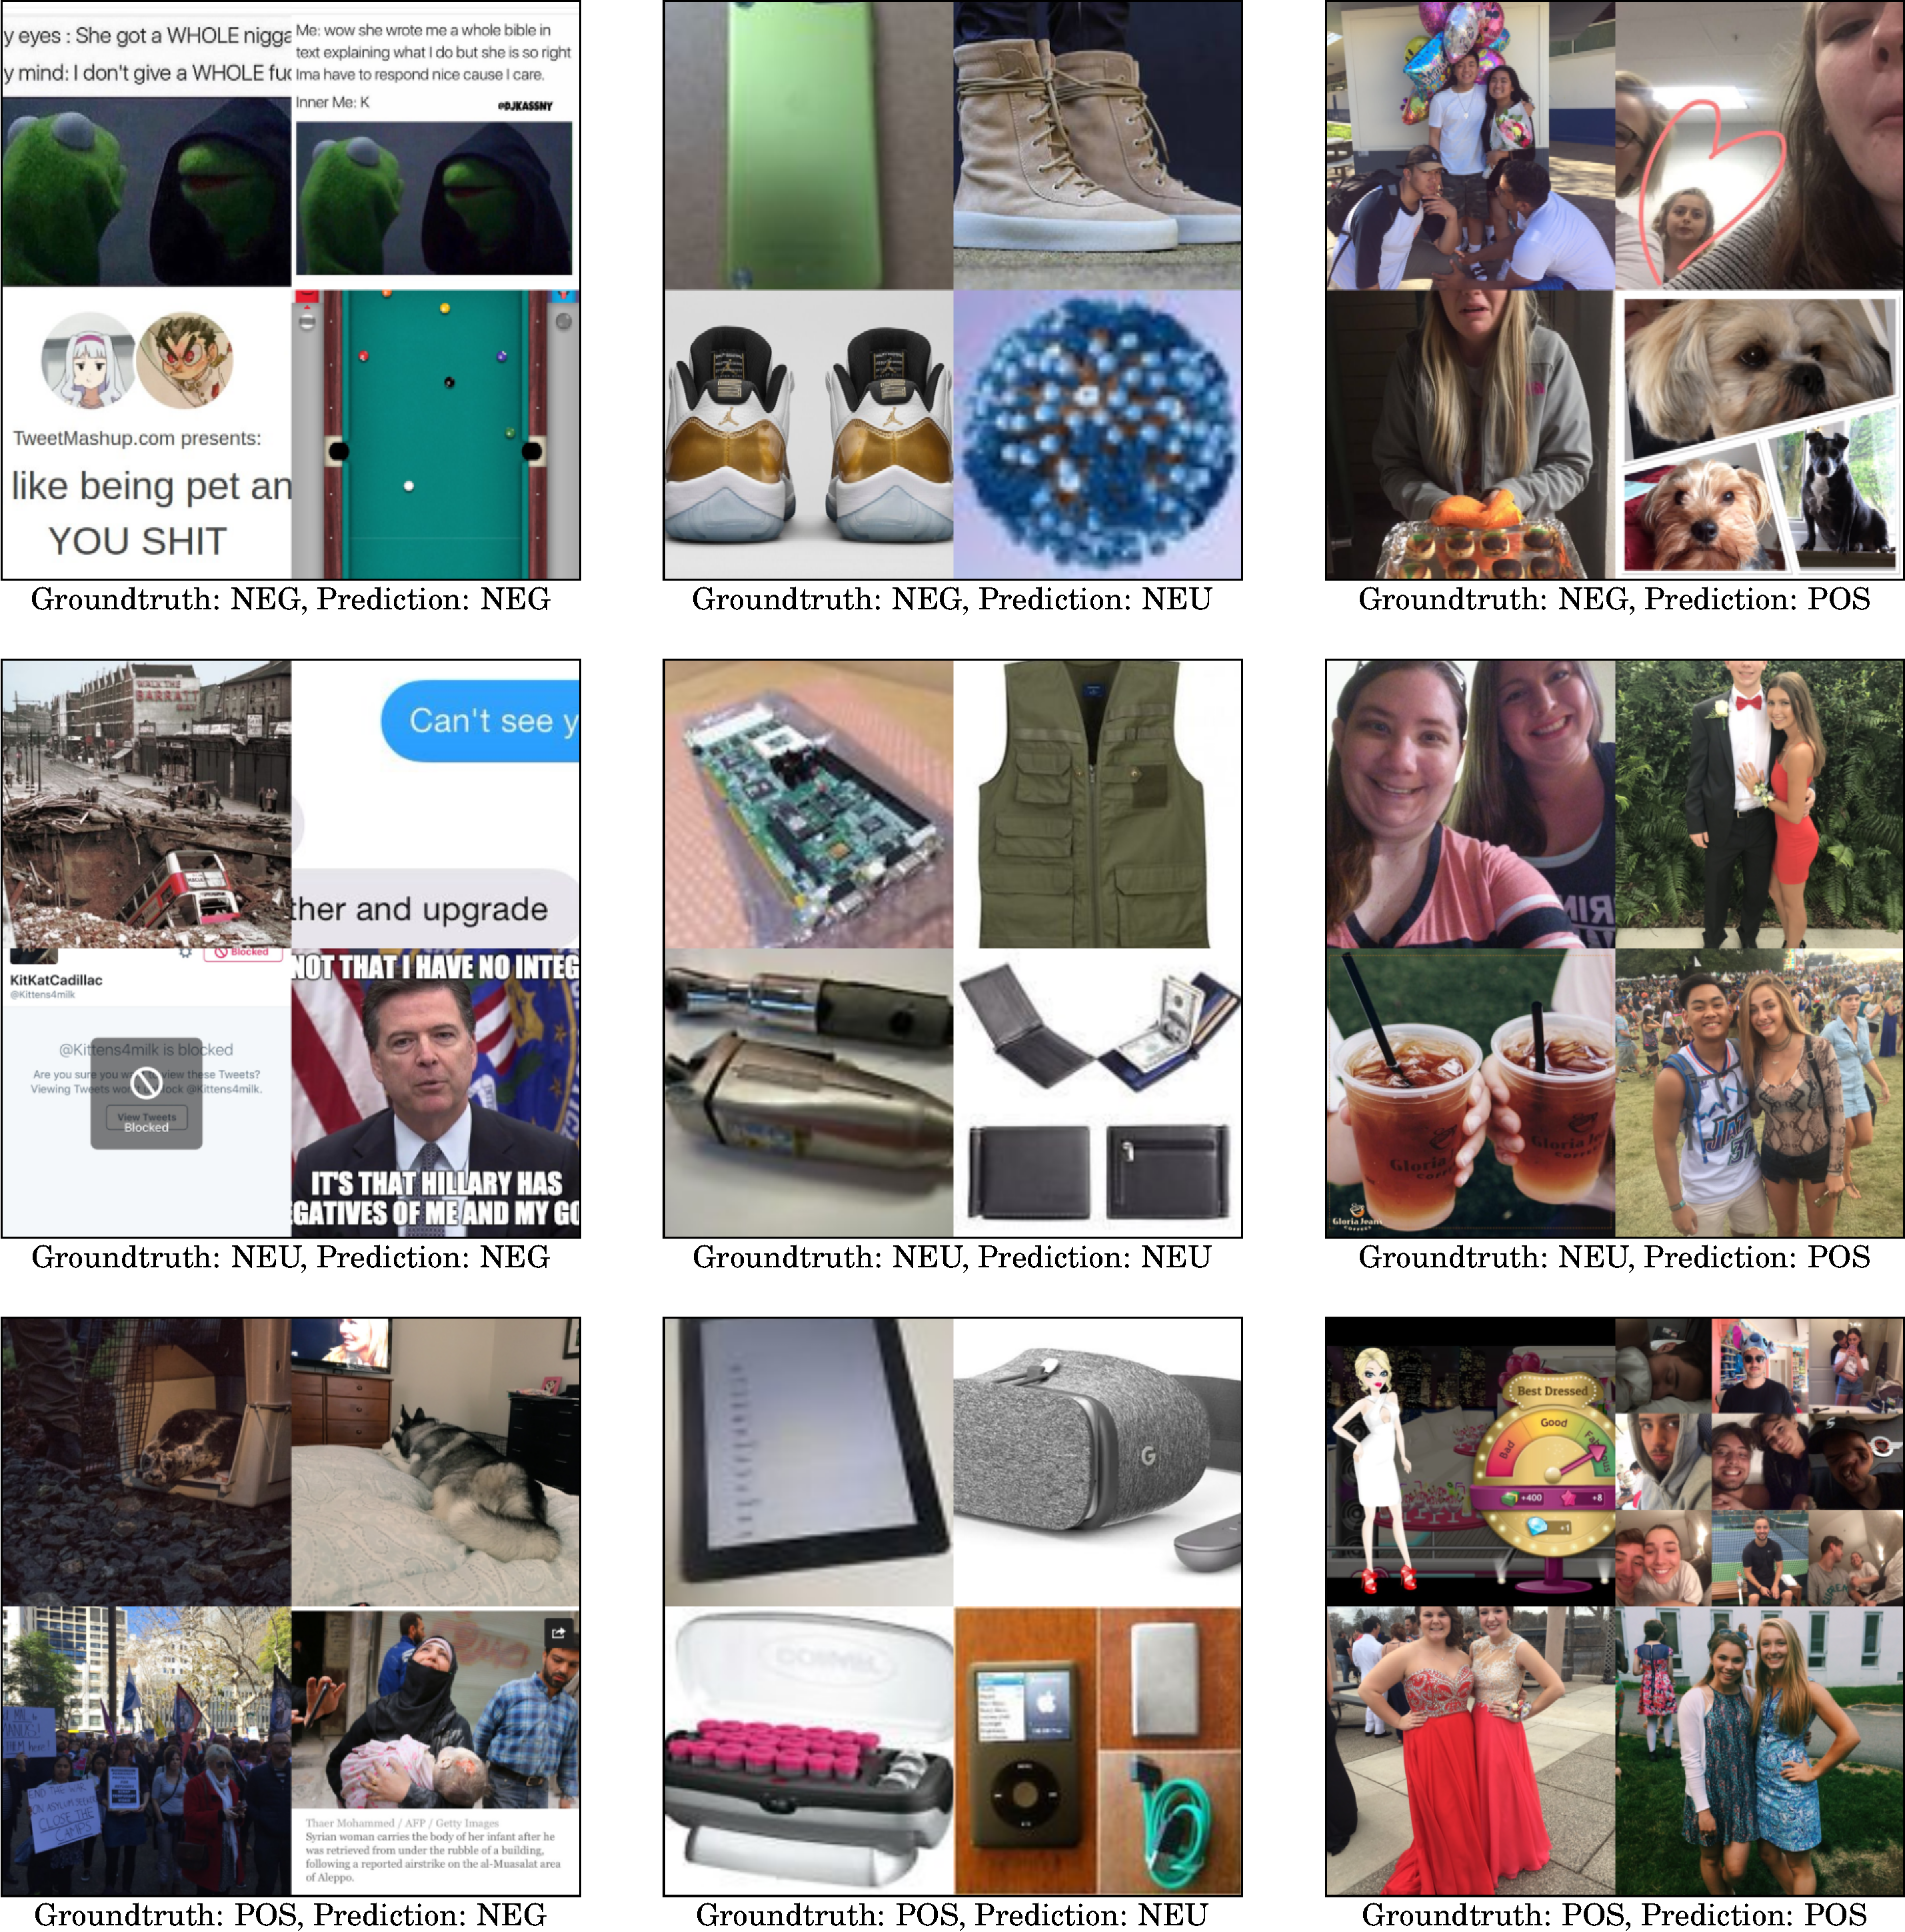
\includegraphics[width=\linewidth]{confusion-images}
\caption{The most confident classifications of our model on our \BTSA\, test set, grouped by all possible (ground-truth, predicted class) couples. Rows (from top to bottom) contains images labeled respectively \emph{negative}, \emph{neutral} and \emph{positive} on the basis of textual sentiment analysis. Columns (from left to right) contain images visually classified respectively as \emph{negative}, \emph{neutral} and \emph{positive} by our model.
%From a qualitative point of view, notice that in several cases the sentiment polarity of the images is better represented by the prediction of our model than the sentiment polarity inferred from the text associated to the images. Since the textual sentiment analysis was used to label both testing and training images, this, on one hand, explains the low accuracy upper bound obtained by our model on the {\BTSA} test set and, on the other hand, confirms that we used sufficiently large set of training data to allow the deep network to handle noisy labels.
}
\label{fig:vsa:confusion-images}
\end{figure}

A considerable amount of works on visual sentiment analysis report the 5-fold cross-validation accuracy on the Twitter Testing Dataset~\cite{campos2017pixels,islam2016visual,li2018image,you2015robust}, in which the prediction of each fold is computed with a model fine-tuned on the other four folds.
In order to compare to those approaches, we also tested our models in this setting, and we reported the 5-fold accuracy obtained in \ref{tab:vsa:fold-results}.
However, we think that this measure is inappropriate for our cross-media approach since it tends to highlight how well a pre-trained model adapts to a specific task or dataset.
In fact, as evidenced by the results, models trained on generic (not sentiment-related) datasets, like AlexNet and VGG-19, not necessarily perform worse than the same models previously fine-tuned on a sentiment-related dataset.
For example our best approach ({\ourFtVGG} FT-A), achieves a 5-fold accuracy of 0.896 on the five agree subset, that corresponds only to an improvement of 1.5\% with respect to VGG-19 trained on a generic dataset.
Moreover, our technique is based on a cross-media approach, i.e., it relies on labels not coming from a visual inspection of the images.
Thus, we think that a fine-tuning of our models on manually labeled images is inappropriate for our goal.
In any case, also in this test setting, our models outperform other state-of-the-art visual classifiers, such as PCNN, DeepSentiBank and MVSO, which were trained on high-quality sentiment-related dataset.

Taken together, these results indicate that our cross-media learning approach is a first important step towards building systems able to learn the sentiment polarity of images autonomously from the Web.

%Differently by other visual sentiment classifiers

% In order to compare the performance of our model to other state-of-the-art methods, we also performed a 5-fold cross-validation on the testing subsets (as also done in~\cite{Campos2016,islam2016visual,li2018image,you2015robust}), in which we compute the prediction of each fold with a model fine-tuned again on the other four folds. Results for 5-fold cross-validation are reported in Table \ref{tab:Twitter882_5fold}.
\begin{table}
\small
\renewcommand{\tabcolsep}{2.7pt}
\newcolumntype{R}{>{\raggedleft\arraybackslash}X}
\begin{tabularx}{\linewidth}{llRRR}
\toprule
                &                           & \multicolumn{3}{c}{\textsc{Twitter Testing Dataset}} \\
                                              \cmidrule(l){3-5}
\textsc{Method} & \textsc{Training Datasets} & \textbf{\footnotesize 5 agree} & \textbf{\footnotesize $\mathbf{\geq 4}$ agree} & \textbf{\footnotesize  $\mathbf{\geq 3}$ agree} \\
\midrule
\multicolumn{5}{l}{\textbf{Approaches without intermediate fine-tuning}} \\
\midrule
GCH~\cite{siersdorfer2010analyzing}              {\footnotesize (from~\cite{you2015robust})} $\ast$  &   -   &   0.684   &   0.665   &   0.66    \\
SentiBank~\cite{borth2013large}  {\footnotesize (from~\cite{you2015robust})} $\circ$ &   -   &   0.709   &   0.675   &   0.662   \\
LCH~\cite{siersdorfer2010analyzing}              {\footnotesize (from~\cite{you2015robust})} $\ast$  &   -   &   0.710   &   0.671   &   0.664   \\
GCH+BoW~\cite{siersdorfer2010analyzing}         {\footnotesize (from~\cite{you2015robust})} $\ast$  &   -   &   0.710   &   0.685   &   0.665   \\
LCH+BoW~\cite{siersdorfer2010analyzing}        {\footnotesize (from~\cite{you2015robust})} $\ast$  &   -   &   0.717   &   0.697   &   0.664   \\
Sentribute~\cite{yuan2013sentribute}   {\footnotesize (from~\cite{you2015robust})} $\circ$ &   -   &   0.738   &   0.709   &   0.696   \\

CNN~\cite{you2015robust} $\bullet$   &   Flickr (VSO)    &   0.783   &   0.755   &   0.715   \\
AlexNet {\footnotesize (from~\cite{campos2017pixels})} $\bullet$   &  \gls{ilsvrc}12   &   0.817   &   0.782   &   0.739   \\
PlaceCNN~\cite{zhou2014learning}                {\footnotesize (from~\cite{campos2017pixels})} $\bullet$   &   Places205    &   0.830   &   -   &   -   \\
GoogleNet~\cite{szegedy2015going}   {\footnotesize (from~\cite{islam2016visual})}  $\bullet$   &   \gls{ilsvrc}12   &   0.861   &   0.807   &   0.787   \\
HybridNet $\bullet$   &   \gls{ilsvrc}12 + Places205   &   0.867   &   0.814   &   0.781   \\
VGG-19 $\bullet$   &   \gls{ilsvrc}12  &   0.881   &   0.835   &   0.800   \\

\midrule
\multicolumn{5}{l}{\textbf{Approaches using an intermediate fine-tuning}} \\
\midrule

PCNN~\cite{you2015robust} $\bullet$   &   Flickr (VSO) + \emph{ft} Flickr (VSO)  &   0.773   &   0.759   &   0.723   \\
DeepSentiBank~\cite{chen2014deepsentibank} {\footnotesize (from~\cite{campos2017pixels})} $\circ$ $\bullet$ &   \gls{ilsvrc}12 + \emph{ft} Flickr (VSO)  &   0.804   &   -   &   -   \\
MVSO [EN]~\cite{jou2015visual}   {\footnotesize (from~\cite{campos2017pixels})} $\circ$ $\bullet$ & DeepSentiBank~\cite{chen2014deepsentibank} + \emph{ft} MVSO-EN~\cite{jou2015visual}  &   0.839   &   -   &   -   \\
\ourFtAlex\, FT-A (Ours) $\bullet$   &   (\gls{ilsvrc}12 + Places205) + \emph{ft} \BTSA    &   0.864   &   0.830   &   0.800   \\
\ourFtAlex\, FT-F (Ours) $\bullet$   &   (\gls{ilsvrc}12 + Places205) + \emph{ft} \BTSA   &   0.873   &   0.832   &   0.810   \\
\ourFtVGG\, FT-F (Ours) $\bullet$   &   (\gls{ilsvrc}12 + Places205) + \emph{ft} \BTSA   &   0.889   &   0.857   &   0.815   \\
\ourFtVGG\, FT-A (Ours) $\bullet$   &   (\gls{ilsvrc}12 + Places205) + \emph{ft} \BTSA &   \textbf{0.896} &  \textbf{0.866}  &   \textbf{0.820}  \\
\midrule
\end{tabularx}
$\ast=$ based on low-level features, $\circ=$ based on mid-level features, $\bullet=$ based on deep learning
%
%\item[$\ast$]  Approch based on low-level features
%\item[$\circ$]  Approch based on mid-level features
%\item[$\bullet$] Approch based on deep learning

\caption{5-Fold Cross-Validation Accuracy of different methods on Twitter Testing Dataset. \emph{tr} stands for `trained'; \emph{ft} stands for `fine-tuned'. Note that in these experiments \emph{all} the deep models are again fine-tuned on four folds of the Twitter Testing Dataset. During cross-validation we fine-tuned all the weights of our FT models.}
\label{tab:vsa:fold-results}
\end{table}

% \subsubsection{Results on Phototweet Sentiment Benchmark(?)} %LUCIA%rivedere il titolo e decidere se inserire gli exp
%~\cite{borth2013large}
% Ground-truth obtained by AMT annotation

%-------------------------------------------------------------------------

\section{Conclusions}
\label{sec:vsa:conclusion}

In this chapter, we tackle the problem of reducing the cost of building datasets for training deep models for image classification.
We proposed a fully automatic cross-media pipeline that builds a weakly-labeled dataset exploiting social media data and its multi-modality that can be used to train deep models drastically reducing the human interaction needed.
We apply our approach in the context of training a visual sentiment classifier from a large set of multimedia data, without the need of human annotators.
We leveraged on textual information associated to Web images --- which is often noisy and ambiguous --- and demonstrated it is still useful for learning robust visual classifiers.
To this scope, we collected and used more than three million tweets, and we experimentally shown that our approach is effective for learning visual sentiment classifier in the wild.
We publicly released all the collected data and our trained models for future research and applications.